\newpage
\subsection{Class Diagram}
\begin{figure}[h]
    \centering
    \includegraphics[width=1.0\textwidth]{Images/Class/diagram.png}
    \caption{Sơ đồ kiến trúc tổng quan}
    \label{fig:architecture-diagram}
\end{figure}

\subsubsection{Quan Hệ Kế Thừa (Inheritance/Generalization)}

\begin{equation*}
\text{User} \xleftarrow{\text{inherits}} \{\text{Renter}, \text{Owner}, \text{Admin}\}
\end{equation*}

\begin{figure}[h]
    \centering
    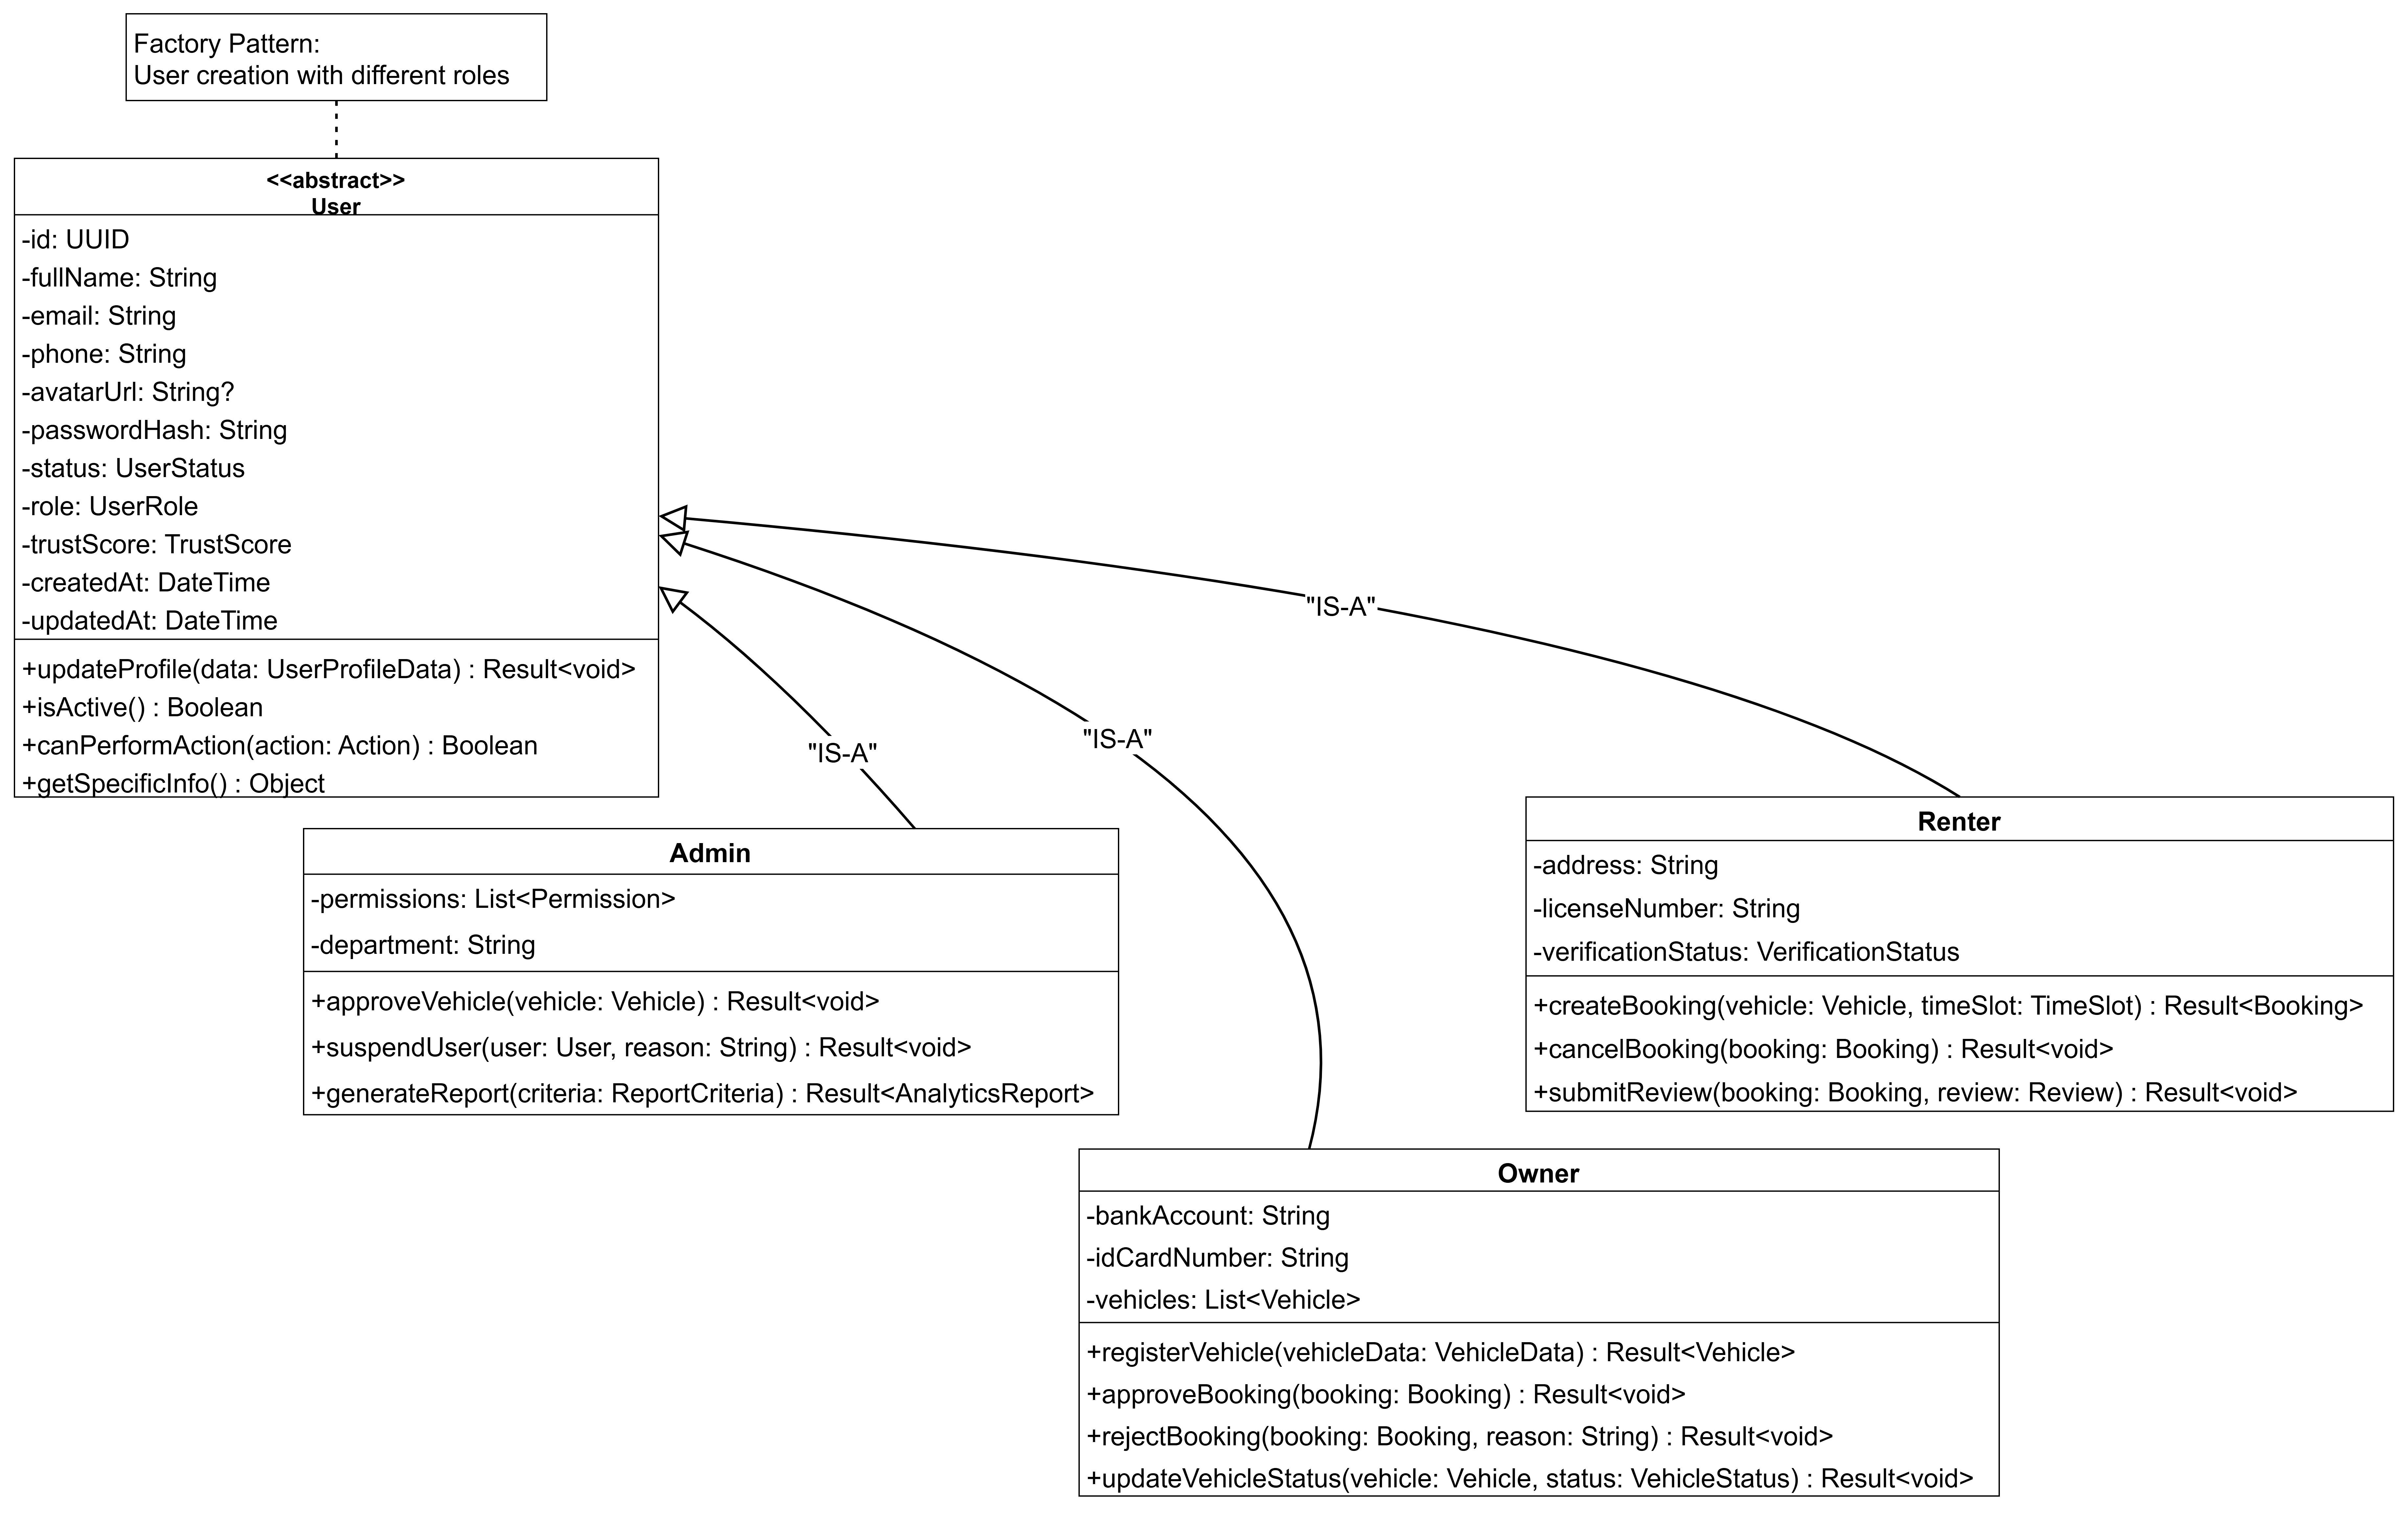
\includegraphics[width=1.0\textwidth]{Images/Class/Inheritance.png}
    \caption{ User là abstract class và các Inheritances}
    \label{fig:Inheritance-class-diagram}
\end{figure}

\begin{itemize}
    \item \textbf{Mô hình phân cấp}: User là abstract class, các role cụ thể kế thừa từ User.
    \item \textbf{Đa hình}: Mỗi role có phương thức \texttt{getSpecificInfo()} riêng.
    \item \textbf{Design Pattern}: Áp dụng \textbf{Factory Pattern} để tạo các loại User.
    \begin{itemize}
        \item {Ưu điểm}: Dễ mở rộng, tuân thủ nguyên lý Open/Closed.
        \item {Triển khai}: Ẩn logic tạo đối tượng phức tạp.
    \end{itemize}
\end{itemize}

\subsubsection{Quan Hệ Hợp Thành (Composition)}

\begin{align*}
\text{User} &\xrightarrow{\text{*--}} \text{TrustScore} \\
\text{Vehicle} &\xrightarrow{\text{*--}} \text{Location} \\
\text{Booking} &\xrightarrow{\text{*--}} \text{TimeSlot} \\
\text{Booking} &\xrightarrow{\text{*--}} \text{Location}_{\text{start}} \\
\text{Booking} &\xrightarrow{\text{*--}} \text{Location}_{\text{end}}
\end{align*}

\begin{itemize}
    \item \textbf{Đặc điểm}:
    \begin{itemize}
        \item Quan hệ ``part-of'' mạnh.
        \item Lifecycle của phần tử phụ thuộc vào đối tượng chính.
        \item Khi đối tượng chính bị hủy → phần tử con cũng bị hủy.
    \end{itemize}

    \item \textbf{Ví dụ}:
    \begin{itemize}
        \item \texttt{User} sở hữu \texttt{TrustScore} (không tồn tại độc lập).
        \item \texttt{Vehicle} có \texttt{Location}.
        \item \texttt{Booking} có \texttt{TimeSlot}.
    \end{itemize}
\end{itemize}

\begin{figure}[h]
    \centering
    \includegraphics[width=0.95\textwidth]{Images/Class/Composition.png}
    \caption{Quan hệ Composition giữa các đối tượng}
    \label{fig:Composition-class-diagram}
\end{figure}


\subsubsection{Quan Hệ Liên Kết (Association)}
\begin{align*}
\text{Owner (1)} &\rightarrow \text{Vehicle (0..*)} \\
\text{Renter (1)} &\rightarrow \text{Booking (0..*)} \\
\text{Vehicle (1)} &\rightarrow \text{Booking (0..*)} \\
\text{Booking (1)} &\rightarrow \text{Payment (0..*)} \\
\text{Booking (1)} &\rightarrow \text{Review (0..1)} \\
\text{User (1)} &\rightarrow \text{Notification (0..*)}
\end{align*}

\begin{figure}[h]
    \centering
    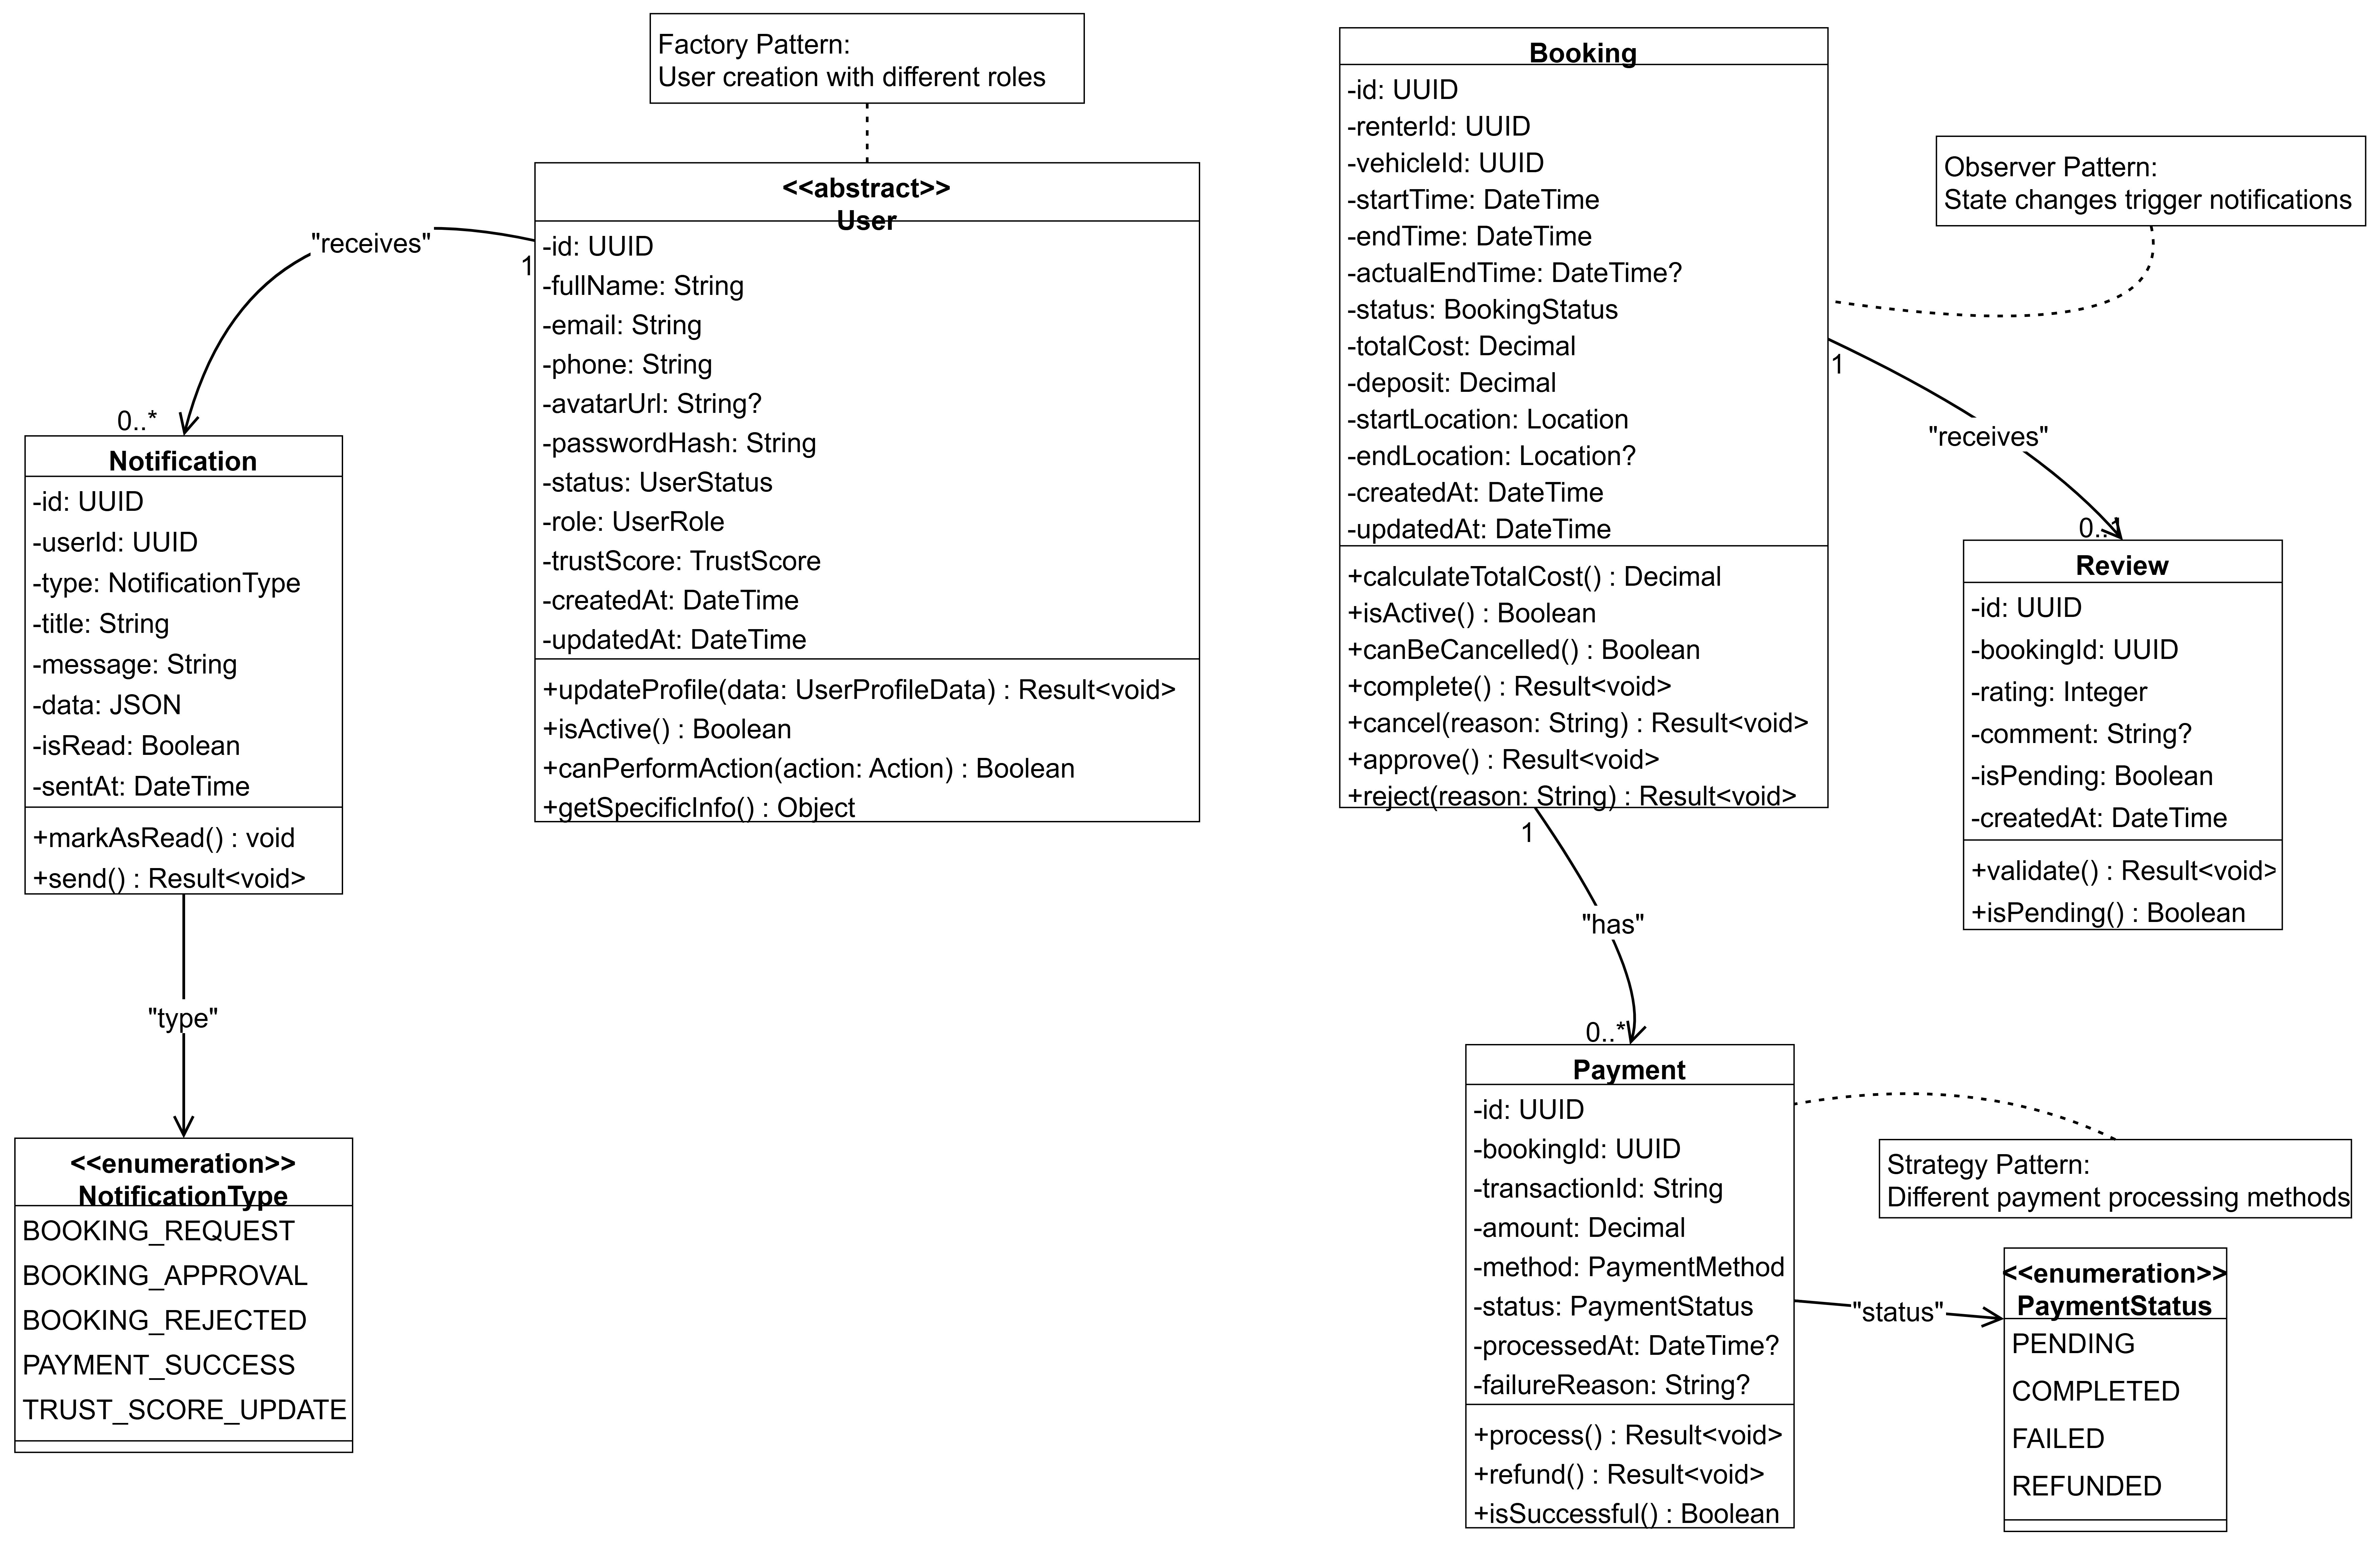
\includegraphics[width=0.95\textwidth]{Images/Class/Association.png}
    \caption{Quan hệ Association giữa các đối tượng}
    \label{fig:Association-class-diagram}
\end{figure}

\begin{itemize}
    \item \textbf{Đặc điểm}:
    \begin{itemize}
        \item Các đối tượng tồn tại độc lập.
        \item Mỗi đối tượng có lifecycle riêng.
        \item Cardinality rõ ràng.
    \end{itemize}

    \item \textbf{Ví dụ}:
    \begin{itemize}
        \item \texttt{Owner → Vehicle}: Chủ có nhiều xe.
        \item \texttt{Vehicle → Booking}: Xe được thuê nhiều lần.
        \item \texttt{Booking → Payment}: Thanh toán liên quan booking nhưng tồn tại riêng.
    \end{itemize}
\end{itemize}

\subsubsection{Quan Hệ Phụ Thuộc (Dependency)}

\begin{itemize}
    \item \textbf{Booking → Payment}:
    \begin{itemize}
        \item Booking phụ thuộc Payment để xử lý giao dịch.
        \item Áp dụng \textbf{Strategy Pattern} cho thanh toán.
    \end{itemize}

    \item \textbf{Review → Booking}:
    \begin{itemize}
        \item Review cần thông tin booking để verify.
    \end{itemize}

    \item \textbf{Notification → User}:
    \begin{itemize}
        \item Notification phụ thuộc vào User để gửi và hiển thị.
        \item Áp dụng \textbf{Command Pattern}.
    \end{itemize}
\end{itemize}

\subsubsection{Các Design Patterns Được Áp Dụng}

\subsubsection*{a. Factory Pattern}

\begin{align*}
\text{UserFactory}: \text{Role} &\rightarrow \text{User} \\
f(\text{RENTER}) &\mapsto \text{Renter instance} \\
f(\text{OWNER}) &\mapsto \text{Owner instance} \\
f(\text{ADMIN}) &\mapsto \text{Admin instance}
\end{align*}

\begin{itemize}
    \item \textbf{Mục đích}: Khởi tạo User theo role.
    \item \textbf{Lợi ích}: Open/Closed, dễ mở rộng, tái sử dụng code.
\end{itemize}

\subsubsection*{b. Observer Pattern}

\begin{equation*}
\text{Booking (Subject)} \xrightarrow{\text{notify}} 
\{\text{Renter}, \text{Owner}, \text{NotificationSystem}\}
\end{equation*}

\begin{itemize}
    \item Giảm coupling giữa các components.
    \item Dễ bổ sung observer mới.
\end{itemize}

\subsubsection*{c. Strategy Pattern}

\begin{align*}
\text{PaymentStrategy} &\supset \{\text{CreditCard}, \text{EWallet}, \text{BankTransfer}\} \\
\text{Payment} &\xrightarrow{\text{uses}} \text{PaymentStrategy}
\end{align*}

\begin{itemize}
    \item Hỗ trợ nhiều phương thức thanh toán.
    \item Tách biệt thuật toán xử lý.
\end{itemize}

\subsubsection*{d. Specification Pattern}

\begin{equation*}
\text{VehicleAvailabilitySpec} = 
f(\text{TimeSlot}) \land g(\text{Location}) \land h(\text{Battery}) \land i(\text{Status})
\end{equation*}

\begin{itemize}
    \item Kết hợp nhiều điều kiện một cách linh hoạt.
    \item Tái sử dụng logic rule.
\end{itemize}

\subsubsection*{e. Command Pattern}

\begin{equation*}
\text{Notification} \xrightarrow{\text{encapsulates}}
\{\text{SendEmail}, \text{SendSMS}, \text{PushNotification}\}
\end{equation*}

\begin{itemize}
    \item Hỗ trợ log, queue, undo.
\end{itemize}

% \subsection{Luồng Nghiệp Vụ Chính}

% \begin{align*}
% \text{Đăng ký xe} &: \text{Owner} \rightarrow \text{Vehicle} \\
% \text{Tạo booking} &: \text{Renter} \rightarrow \text{Booking} \\
% \text{Phê duyệt} &: \text{Owner} \rightarrow \text{Booking} \rightarrow \text{Notify} \\
% \text{Thanh toán} &: \text{Payment} \rightarrow \text{PaymentStrategy} \\
% \text{Hoàn tất} &: \text{Review} \rightarrow \text{TrustScore} \\
% \text{Thông báo} &: \text{Notification} \rightarrow \text{User}
% \end{align*}
